\documentclass{article}
\usepackage[utf8]{inputenc}
\usepackage{amsmath}
\usepackage{graphicx}
\usepackage{float}
\usepackage{amssymb}
\usepackage{listings}
\usepackage{pgfplots}
\usepackage{siunitx}

\usepackage{tabularx}
\usepackage{ragged2e}
\usepackage{multirow}

\pgfplotsset{compat=1.15}
\title{ITIA Target Programming (Robot) Lab Report}
\author{Stefan Adelmann (01633044) and Hannes Brantner (01614466)}
\begin{document}
\maketitle{}
\clearpage{}
\section{SysML Review}
Since the robot station was already designed in an singular SysML description, no two projects had to be merged in this stage. As a review two parts of the description where modified in this phase.

\subsection{Parametric diagram}
The parametric diagram described the calculation of the line distance between two points in 3D space. This calculation however is not part of the user programmable environment for the robot arm. The movement of the arm is controlled by internal algorithms that maximize the efficiency of the robot. Due to the building characteristics of an robot arm the most efficient way is not a straight line, rendering the distance calculation presented in phase 1 obsolete. To create a streamlined description the parametric diagram was removed in phase 2, leaving only relevant diagram types.

\subsection{Internal Block Diagram}
The internal block diagram should display the connectivity between components. For the programming part it would be required in reality to model this down to the individual components of the station, like for example the spring push out piston. This was omitted and abstracted in the description by only specifying the connectors that are present on the robot. If a developer needs to know the pin that is used for a specific part a chart or specification of the connector standard can be found in the datasheet of the robot controller. The internal block diagram is therefore regarded as the viewpoint of a system integrator that needs to connect modules but not individual components.

\subsection{Assignment addition}
In phase 2 of this lab it was required to implement an OPC UA interface that can be used to control certain aspects of the robot without it running a specific program. For this a Raspberry Pi running an OPC UA server was added to the robot station. This change can be seen in the Functional Requirements where the control capabilities were added as a requirement that needs to be satisfied by the controller, as well as in the block and internal block diagram were the component was added to the right place. Since the actual assembly process is still carried out the same way and only external controls were added the behavioral diagrams stay the same as in phase 1.
\section{I/O Mapping}
The Robot station primarily consists of the robot arm with a multi-functional gripper and sensors and actuators located in two modules. Since the robot arm is specifically connected and controlled by the robot controller it is separated in this report from the I/Os of the other two modules namely the assembly and handling stations. 

\subsection{Robot}
The location of the robot arm in 3D space is controlled by 6 freedom axis. It is important to note that the coordinate system of the robot can be changed on the controller. For this report the XYZ mode was chosen. The basis of the coordinate system can be seen in \ref{fig:robot_axis}. The first 3 parameters of the move command shown in \ref{tab:robot_ctrl} specify the X, Y, and Z coordinate of the arm. The last 3 A, B, C describe rotations around the coordinate system axis. In XYZ mode the basis of rotation is the same as the basis of the xyz coordinate system. In other movement modes this however can be changed, a thorough list of coordinate system modes can be found in the datasheet of the robot controller.\newline
Due to the inherent collision danger embossed by the remote connection and camera angle it was not safely possible to test all movement patterns of the robot. The move commands shown in \ref{tab:robot_ctrl} where however tested by entering precollected arm positions that where known to be collision free.
\begin{figure}[htp]
	\centering
	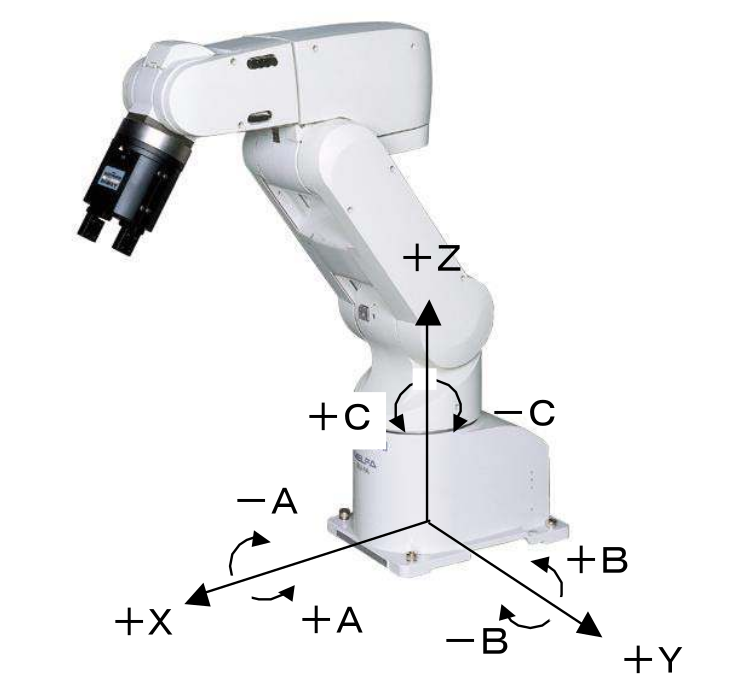
\includegraphics[width=0.6\textwidth]{images/robot_axis.png}
	\caption{Robot coordinate system in XYZ mode}
	\label{fig:robot_axis}
\end{figure}
\par Additional to the movement commands in the robot programming language Melfa-V, methods running on an OPC UA server where implemented in this phase. A detailed description of these methods can be found in section 3 of this report.
\begin{center}
	\setlength\extrarowheight{4pt}
	\small
		\begin{tabularx}{\textwidth}{|p{3cm}|p{4cm}|X|}
			\hline
			\multicolumn{3}{|c|}{\bf \color{white} \large Gripper}\\
			\hline\hline
			\bf Melfa-Command & \bf OPC UA & \bf Beschreibung\\
			\hline\hline
			Mov(X,Y,Z,A,B,C) & move(X,Y,Z,A,B,C) & Modul Roboter (Hand) - Position, Rotation anfahren\\
			\hline
			HOpen 1 & gripperOpen() & Modul Roboter (Hand) - Gripper öffnen\\
			\hline
			HClose 1 & gripperClose() & Modul Roboter (Hand) - Gripper schließen\\
			\hline
		\end{tabularx}
		\label{tab:robot_ctrl}
\end{center}

\subsection{Robot Control}
The robot itself as well as the modules present in the robot station are controlled by a robot controller. Programming is done via the programming language Melfa-V. Connection with the controller can be established via the parameters shown in table \ref{tab:controller}. 
\begin{center}
		\begin{tabular}[h]{|p{1.2cm}p{5.5cm}|}
			\hline
			\multicolumn{2}{|c|}{\bf Controller}\\
			\hline\hline
			Device: & Robot Controller\\
			\hline
			ID: & CR750-D\\
			\hline
			MAC: & \\
			\hline
			IP: & 192.168.162.82/25\\
			\hline
		\end{tabular} \\
		\label{tab:controller}
\end{center}
To gain the possibility of integrating the robot station into the other station in this lab, an OPC UA server running on a Raspberry Pi was improved in this phase. Connection to this server can be established via the parameters shown in table \ref{tab:robot_raspi}.
\begin{center}
	%\scriptsize
	\setlength\extrarowheight{2pt}
			\begin{tabular}[h]{|p{1.2cm}p{4.5cm}|}
			\hline
			\multicolumn{2}{|c|}{\bf OPC UA Gateway}\\
			\hline\hline
			Device: & RaspberryPi 3\\
			\hline
			ID: & BCM2835 (a02082)\\
			\hline
			MAC: & b8:27:eb:09:db:ca\\
			\hline
			IP: & 192.168.162.84/25\\
			\hline
			Port: & 4840\\
			\hline
		\end{tabular} 
		\label{tab:robot_raspi}
\end{center}
\newpage
\subsection{Sensors/Actuators}
The sensors and actuators are connected to the robot controller via the connectors shown in the internal block diagram of the SysML description. On the software side of the controller inputs and outputs are addressed by an index. As it can be seen in the tables \ref{tab:robot_sensor} and \ref{tab:robot_actuator}, there is not distinction between input and output purely by looking at the index. This is handled in Melfa-V by two different function calls, \texttt{M\_out(0)} will address output at index 0 while \texttt{M\_In(0)} will address the input.
\begin{center}

	\setlength\extrarowheight{4pt}
	\small
	\begin{tabularx}{\textwidth}{|p{1cm}|X|}
		\hline
		\multicolumn{2}{|c|}{\bf \color{black} \large Sensoren}\\
		\hline\hline
		\bf Index & \bf Beschreibung\\
		\hline\hline
		1 & Modul Roboterhandling - Werkstück ausgerichtet\\
		\hline
		2 & Modul Roboterhandling - Werkstück in Abholposition\\
		\hline
		3 & Bedienfeld - Start (Schließer)\\
		\hline
		4 & Bedienfeld - Stopp (Öffner) \\
		\hline
		5 & Bedienfeld - Reset (Schließer)\\
		\hline
		7 & Bedienfeld - COM Brücke (I7)\\
		\hline
		8 & Modul Robotermontage (Federmagazin) - Schieber eingefahren\\
		\hline
		9 & Modul Robotermontage (Federmagazin) - Schieber ausgefahren\\
		\hline
		10 & Modul Robotermontage (Federmagazin) - Feder vorhanden \\
		\hline
		12 & Modul Robotermontage (Deckelmagazin) - Schieber eingefahren\\
		\hline
		13 & Modul Robotermontage (Deckelmagazin) - Schieber ausgefahren\\
		\hline
		15 & Modul Robotermontage (Deckelmagazin) - Deckel auf Ablage\\
		\hline
		900 & Modul Roboter (Hand) - Teil nicht schwarz\\
		\hline
	\end{tabularx}
\label{tab:robot_sensor}
\end{center}
The color sensor shown in the last line of table \ref{tab:robot_sensor} is in a different index range as the other inputs, this is caused by its location on the robot arm itself. These inputs and subsequently the outputs of the arm are already predefined in the controller software, while the function of the general purpose pins of the other sensors and actuators can be chosen by the developer.\newline
It can be seen in both tables that indices are missing. These missing pins are connected to boards on the robot station modules but not assigned any function. If the robot station is improved, this in and outputs can be used.

\begin{center}
	\setlength\extrarowheight{4pt}
	\small
	\begin{tabularx}{\textwidth}{|p{1cm}|X|}
		\hline

		\multicolumn{2}{|c|}{\bf \color{black} \large Aktoren}\\
		\hline\hline

		\bf Index & \bf Beschreibung\\
		\hline\hline
		0 & Bedienfeld - Start (LED)\\
		\hline
		1 & Bedienfeld - Reset (LED)\\
		\hline
		2 & Bedienfeld - Q1 (LED)\\
		\hline
		3 & Bedienfeld - Q2 (LED)\\
		\hline
		4 & Bedienfeld - COM Brücke (Q4)\\
		\hline
		8 & Modul Robotermontage (Federmagazin) - Schieber ausfahren\\
		\hline
		12 & Modul Robotermontage (Deckelmagazin) - Schieber ausfahren\\
		\hline
	\end{tabularx}
	\label{tab:robot_actuator}
\end{center}
\newpage

\section{Handover Protocol}
In the robot station the whole operation is carried out by one controller, a handover protocol is therefore not needed to implement the assembly process. The robot could however be integrated into the other stations in another role. For this use case, a previous bachelor thesis implemented a basic interface for controlling the robot via OPC UA. In its original form it was for example possible to start and stop the operation of the robot. In this phase this server was updated and new methods where added.\newline
The methods that were implemented are shown in table \ref{tab:robot_opc}. By calling these methods in combination with the tables provided in the previous section a different controller like one of the PLCs in this lab can control the robot via the OPC UA interface.
\begin{center}
	\setlength\extrarowheight{4pt}
	\small
	\begin{tabularx}{\textwidth}{|p{5cm}|X|}
		\hline
		
		\multicolumn{2}{|c|}{\bf \color{black} \large Methods}\\
		\hline\hline
		
		\bf Method & \bf Function\\
		\hline\hline
		OpenGripper() & Opens the multi function gripper\\
		\hline
		CloseGripper() & Closes the multi function gripper\\
		\hline
		Move(X,Y,Z,A,B,C) & Moves the robot arm to the given coordinates\\
		\hline
		GetErrorLog(NUMLOGS) & Returns the last NUMLOGS errors that occurred\\
		\hline
		ReadInput(INDEX) & Returns the state of the input at the given index\\
		\hline
		WriteOutput(INDEX, STATE) & Sets the output at the given INDEX to the given STATE\\
		\hline
		ResetError() & Resets the robot controller from the error state\\
		\hline
	\end{tabularx}
\label{tab:robot_opc}
\end{center}
While it is possible with these methods to implement the assembly behavior of the demo robot implementation certain settings like the coordinate system have to be done manually, otherwise the move command could crash.\newline
In addition to the active control methods, two important error methods were implemented. During use of the robot arm, internal safeguards of the robot arm or syntax errors will switch the robot into error mode preventing its use. \texttt{ResetError()} can be used to revert the robot into its operational state. A list of the last errors can be retrieved with the \texttt{GetErrorLog(NUMLOGS)}. A call will return the last NUMLOGS errors, with additional information like timestamp, error-code and error text and in which program/line the error occurred.
\end{document}
